\documentclass[border=10pt]{standalone}
\usepackage[svgnames]{xcolor}
\usepackage{amsmath}
\usepackage{pgfplots}
\pgfplotsset{compat=newest}
\usepackage[sfdefault]{FiraSans}
\usepackage{FiraMono}
\renewcommand*\familydefault{\sfdefault}
\begin{document}
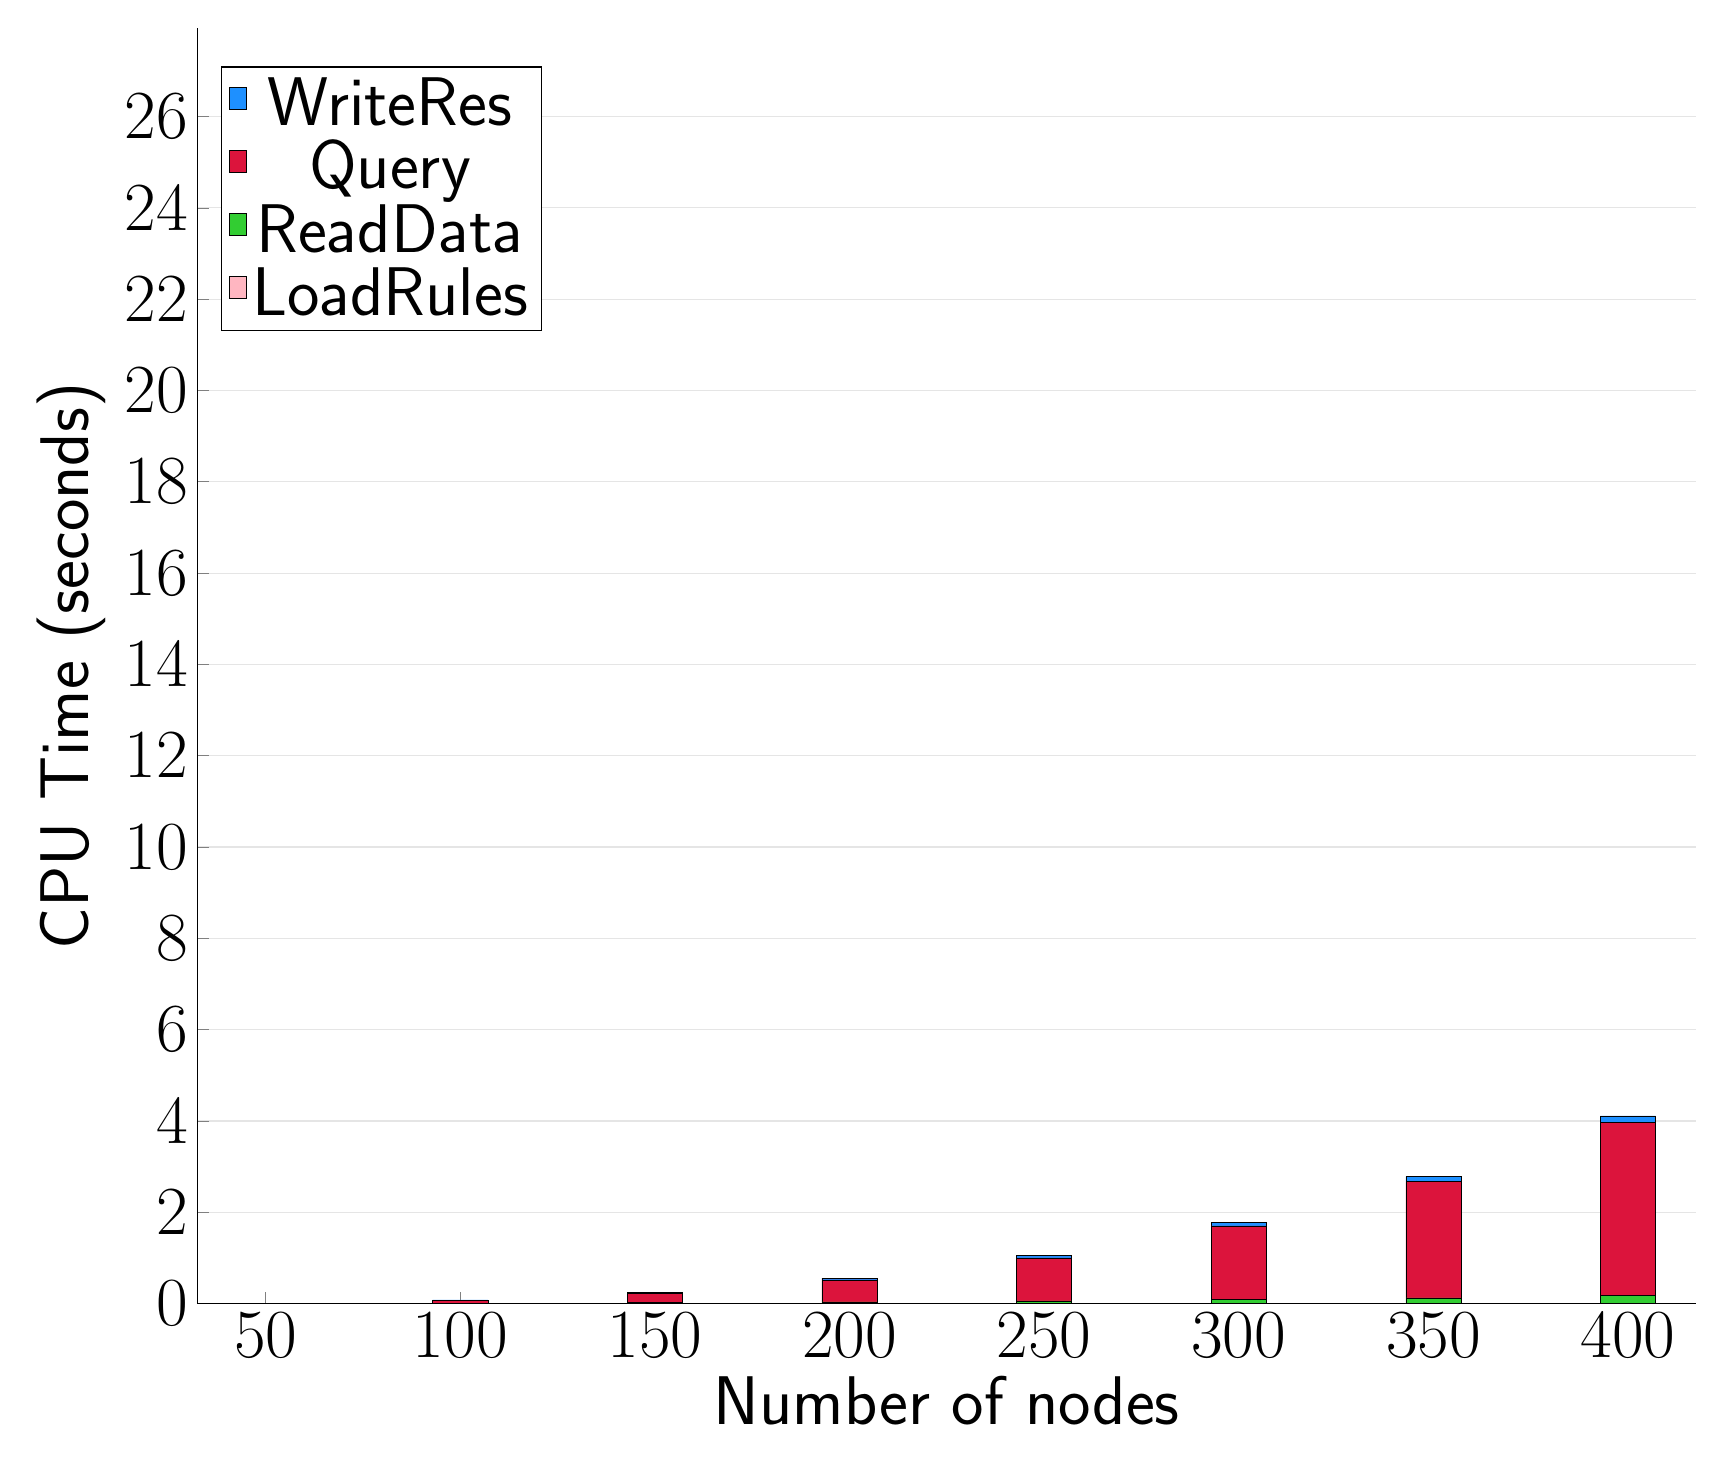
\begin{tikzpicture}
\begin{axis}[
   ybar stacked,
   width=1.7\textwidth,
   bar width=0.7cm,
   ymajorgrids, tick align=inside,
   major grid style={draw=gray!20},
   xtick=data,
   ymin=0, ymax=27.933910000000004,
   axis x line*=bottom,
   axis y line*=left,
   enlarge x limits=0.05,
   legend style={
       at={(0.23, 0.97)},
       anchor=north east,
       legend columns=1,
       font=\Huge,
   },
   ylabel={CPU Time (seconds)},
   xlabel={Number of nodes},
   label style={font=\Huge},
   tick label style={font=\Huge},
]
\addlegendimage{fill=DodgerBlue, draw=black, line width=0.2pt}
\addlegendentry{WriteRes}
\addlegendimage{fill=Crimson, draw=black, line width=0.2pt}
\addlegendentry{Query}
\addlegendimage{fill=LimeGreen, draw=black, line width=0.2pt}
\addlegendentry{ReadData}
\addlegendimage{fill=LightPink, draw=black, line width=0.2pt}
\addlegendentry{LoadRules}
\addplot +[fill=LightPink, draw=black, line width=0.2pt] coordinates {
(50, 0.0006185000000000001)
(100, 0.0006165999999999998)
(150, 0.0005919)
(200, 0.0006088000000000002)
(250, 0.0006273000000000003)
(300, 0.0006271000000000004)
(350, 0.0006229)
(400, 0.0006426000000000003)
};
\addplot +[fill=LimeGreen, draw=black, line width=0.2pt] coordinates {
(50, 0.0022533)
(100, 0.008968100000000001)
(150, 0.020756)
(200, 0.0381426)
(250, 0.061549900000000005)
(300, 0.09132929999999999)
(350, 0.126653)
(400, 0.171447)
};
\addplot +[fill=Crimson, draw=black, line width=0.2pt] coordinates {
(50, 0.0076763)
(100, 0.0606592)
(150, 0.2059825)
(200, 0.4827714)
(250, 0.940304)
(300, 1.6085115)
(350, 2.5452947999999997)
(400, 3.8049542)
};
\addplot +[fill=DodgerBlue, draw=black, line width=0.2pt] coordinates {
(50, 0.0024341000000000002)
(100, 0.0092322)
(150, 0.019923299999999998)
(200, 0.0353161)
(250, 0.0558608)
(300, 0.0779628)
(350, 0.10887960000000008)
(400, 0.13417229999999997)
};
\end{axis}
\end{tikzpicture}

\end{document}
